Avant de créer les liens entre les \textit{exempla} et les encyclopédies, il était essentiel d’identifier précisément les citations d'encyclopédies qui contiennent des \textit{exempla} et les récits exemplaires qui s'appuient sur ces \index{Encyclopédies}encyclopédies. Pour cela, j'ai ajouté un champ de recherche spécifique dans ThEMA et  un nom d'autorité a été ajouté dans SourcEncyMe par Emmanuelle Kuhry. J'ai également envisagé de comparer les textes entre ThEMA et SourcEncyMe pour repérer les réemplois d'encyclopédies dans SourcEncyMe et les \textit{exempla} dans ThEMA. En fin de compte, le repérage s'est principalement appuyé sur des mots-clés signalant les \textit{exempla} dans SourcEncyMe et sur la présence de mentions d'encyclopédies déjà indexées dans ThEMA.


\section{Création d'outils pour chercher dans les données qui seront connectées}
Pour faciliter l'accès des utilisateurs aux informations ayant aidé à faire des liens, des outils spécifiques dans les deux bases de données ont été mis en place.

\

Dans SourcEncyMe, tous les \textit{exempla} ont été catégorisés sous un même nom d'autorité (\textit{Exemplum}) par \index{Emmanuelle Kuhry}Emmanuelle Kuhry, même s'ils ne peuvent pas être entièrement considérés comme tels car chaque récits exemplaire peut être considéré comme œuvre à part entière\footnote{Cette autorité est désignée par un titre standardisé appelé entité canonique. \cite{SourcEncyMe}}. Ce choix a été guidé par des contraintes techniques : toutes les sources de la base sont balisées de manière uniforme, et pour éviter de créer un nouveau système de balisage, le balisage existant a été adapté pour inclure les \textit{exempla}. Ainsi, contrairement à ThEMA, où une distinction est faite entre différents types de récits, SourcEncyMe utilise le terme générique « exemplum » pour tous les \index{Récits exemplaires}récits exemplaires\footcite{InformationsThEMA}. \\

\begin{lstlisting}[breaklines=true]
	<cit xml:id="cit_idp94946128" n="11">
		<bibl>
			<ref target="#exemplum">Exemplum</ref>
		</bibl>
		<quote>Item activa vita assimilatur colli, primo, propter ordinem
		prioratus : est enim collis pes montis. Nam per collem ascendimus ad montem, quia scilicet per vitam activam ad contemplativam venimus. <name type="personne">Iacob</name> enim post <name type="personne">Lie</name> connubium (per quam activa vita signatur) ad <name type="personne">Rachaelis</name> pervenit amplexum, per quam contemplative vite formositas figuratur.</quote>
	</cit>
\end{lstlisting}

Grâce à ce système, les utilisateurs peuvent avec un champ de recherche spécifique, qui existait déjà avant mon stage, rechercher tous les \textit{exempla} présents dans les \index{Encyclopédies}encyclopédies en saisissant « exemplum » dans le champ « Œuvre » : \\

\begin{figure}[H]
	\centering
	\fbox{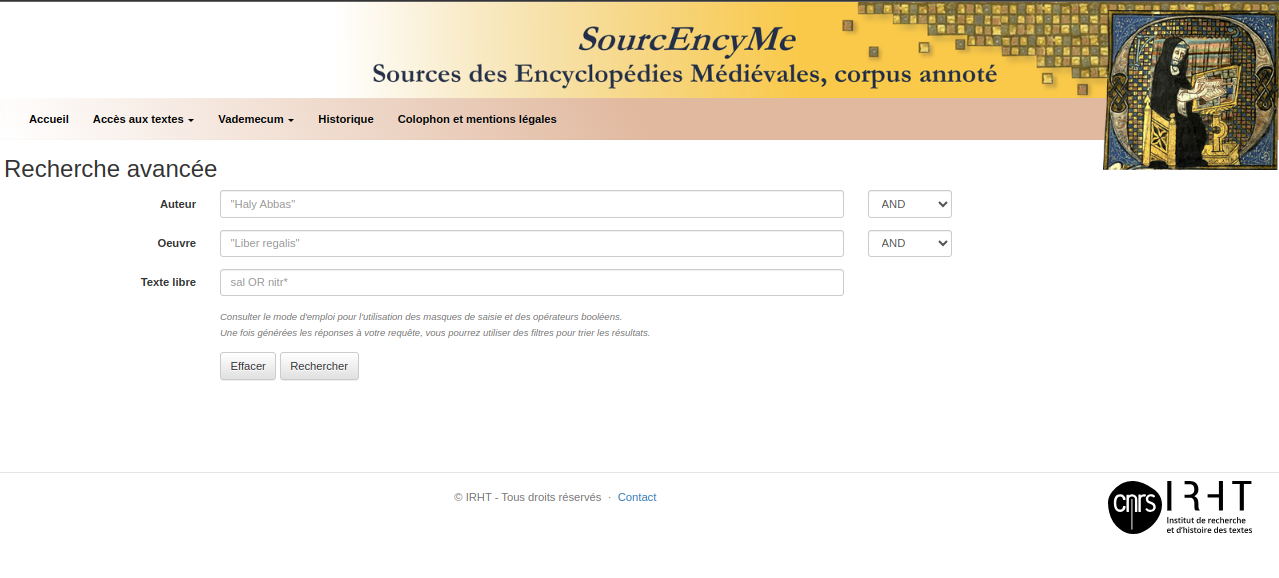
\includegraphics[width=0.8\linewidth]{images/champrecherchesourcencyme.png}}
	\caption{Champ de recherche dans SourcEncyMe}
\end{figure}

Dans ThEMA, en revanche, il a été nécessaire de créer un champ de recherche spécifique pour permettre aux utilisateurs d'explorer les sources et les textes apparentés. Bien que ces informations soient déjà visibles, il n'était pas possible de les rechercher directement. Pour remédier à cela, j'ai modifié le fichier « search.xql » situé dans le dossier « modules » de la base de données. J'ai adapté le code de recherche en texte intégral, initialement prévu pour les résumés des \index{Récits exemplaires}récits exemplaires, afin de permettre la recherche dans les sources et les textes apparentés (annexe F). \\

\begin{figure}[H]
	\centering
	\fbox{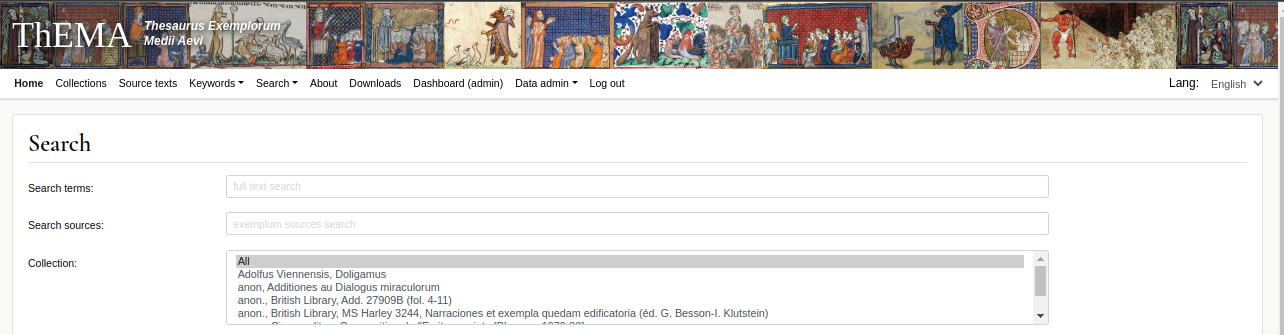
\includegraphics[width=0.8\linewidth]{images/champrecherchethemasource.png}}
	\caption{Nouveau champ de recherche dans ThEMA}
\end{figure}

Toutefois, le développement de ce code n'a pas pu être finalisé avant la fin de mon stage. En l'état, le code affiche l'ensemble des \textit{exempla} en haut de la page ainsi que les résultats de recherche dans les sources et textes apparentés en bas, alors qu'il aurait dû se limiter à afficher uniquement ces derniers. \\

\begin{figure}[H]
	\centering
	\fbox{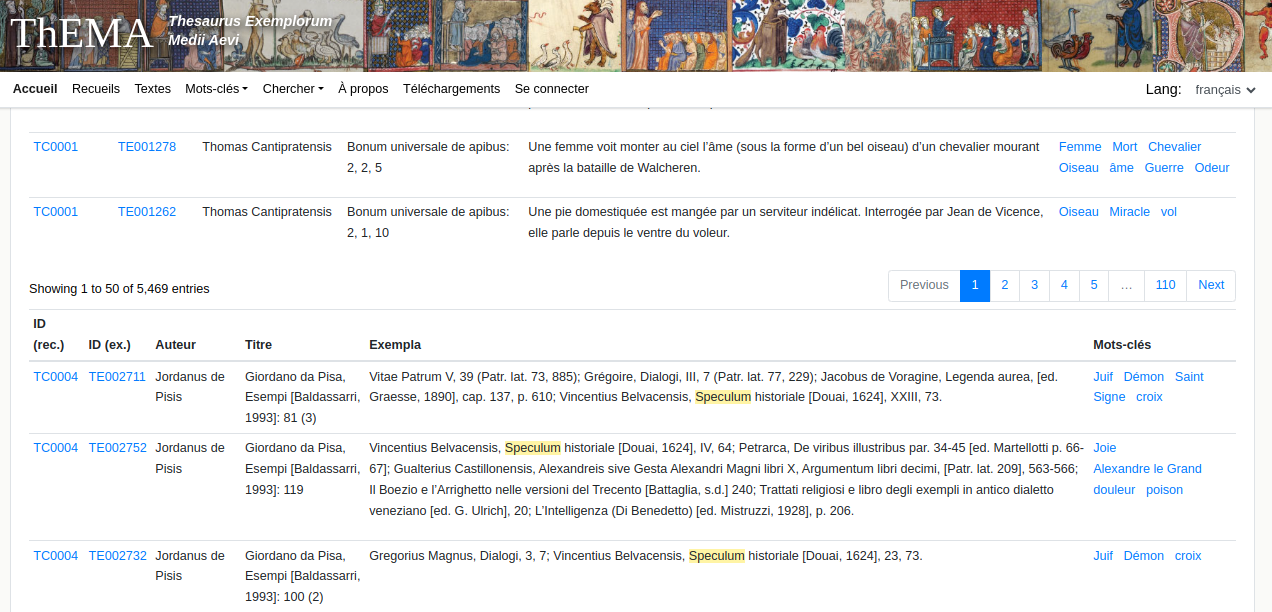
\includegraphics[width=0.8\linewidth]{images/pugthema.png}}
	\caption{Résultat du nouveau champ de recherche dans ThEMA}
\end{figure}

\section{Identification des liens par comparaison des textes}
Après avoir mis en place ces outils pour faciliter la recherche d'\textit{exempla}` et d'\index{Encyclopédies}encyclopédies dans ThEMA et SourcEncyMe, j'ai également exploré la possibilité d'utiliser des méthodes plus avancées pour affiner encore davantage cette analyse et trouver des liens qui n'ont pas encore été repérés. C'est ainsi que j'ai envisagé l'utilisation de l'intelligence artificielle pour comparer les textes des deux bases de données. L'idée était de tirer parti de la rapidité et de la précision de l'IA pour détecter non seulement les \textit{exempla} dans SourcEncyMe, mais aussi pour identifier des mentions d'encyclopédies supplémentaires dans ThEMA, au-delà de celles déjà repérées lors de l'indexation initiale.

Toutefois, cette approche s'est rapidement heurtée à plusieurs défis. Le premier obstacle provenait d'une différence importante entre les deux bases de données. ThEMA, pour des raisons de droits d'auteur, ne peut fournir que de courts résumés en français des \index{Récits exemplaires}récits exemplaires, tandis que SourcEncyMe donne accès aux textes complets en latin, car des éditions récentes n'existent pas forcément. Cette disparité linguistique a rendu l'utilisation de l'intelligence artificielle complexe, nécessitant la traduction des textes des \index{Encyclopédies}encyclopédies en français pour permettre une comparaison efficace\footnote{Je n'ai pas trouvé de modèles de langues entraînés pour le latin. De toute manière, ThEMA ne possèdent qu'un nombre limité de récits où le texte latin et indiqué}.\\

\begin{figure}[H]
	\centering
	\fbox{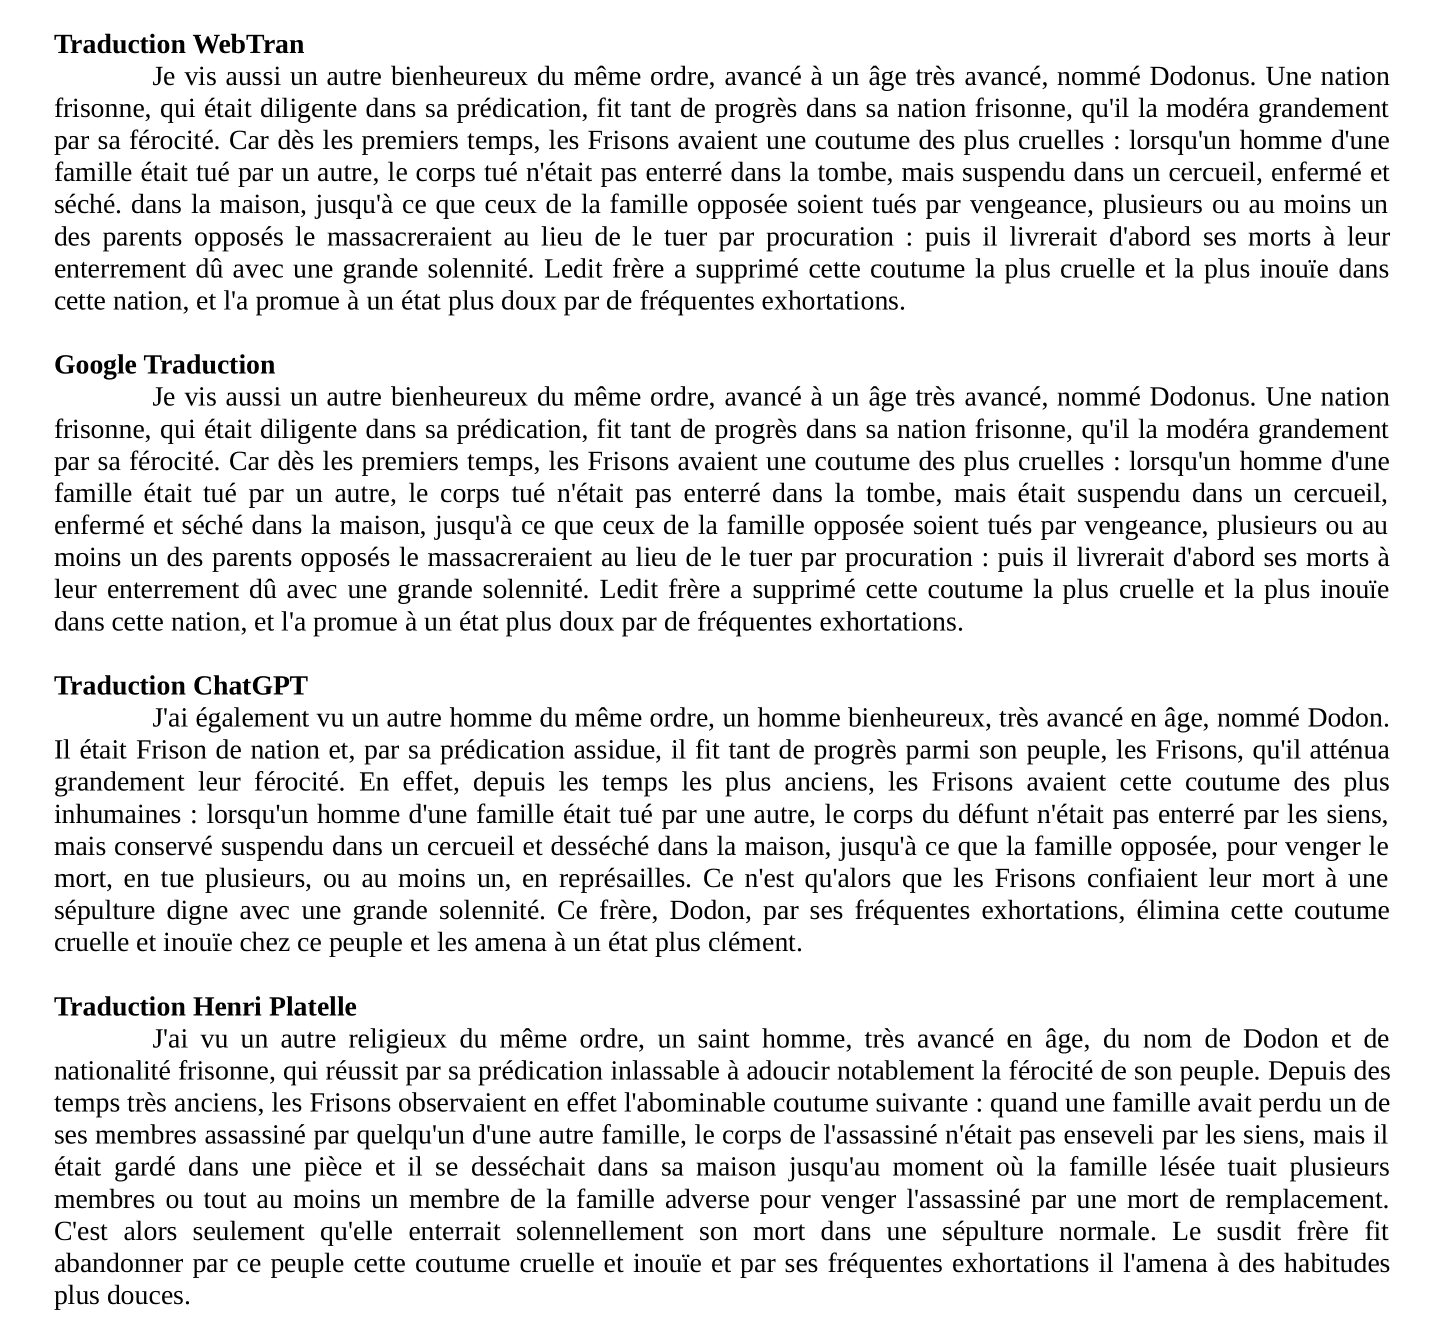
\includegraphics[width=0.8\linewidth]{images/tradlang.png}}
	\caption{Différentes traductions d'un même \textit{exemplum}}
\end{figure} 

La traduction elle-même a posé des problèmes. Malgré plusieurs tentatives, je n'ai trouvé aucun traducteur en ligne parfaitement fiable. Parmi les outils testés, ChatGPT se distinguait légèrement de Google Traduction et de WebTran, mais ces outils imposaient des restrictions sur le web scraping, la technique d'extraction automatisée de données à partir de sites web. Pour ChatGPT, l'achat de jetons était requis pour accomplir cette tâche, tandis que Google Traduction et WebTran interdisaient explicitement le web scraping dans leurs conditions d'utilisation, compliquant encore davantage le processus.

En fin de compte, la solution retenue a été de traduire manuellement, ou partiellement, les textes des \index{Encyclopédies}encyclopédies en m'appuyant sur des ressources en ligne. Bien que la traduction reste imparfaite, un code que j'ai développé (annexe G) a permis de repérer certaines similitudes entre les textes. Cependant, même avec des optimisations, ce traitement s'est révélé extrêmement lent : chaque comparaison prenait environ 20 minutes, en raison du volume important de données à analyser.

\

Le code, bien qu'imparfait, s'est montré relativement efficace. Lors d'un test visant à trouver les nombreuses équivalences de l'\textit{exemplum} de la « moniale chaste mais bavarde »\footcite{RecitsExemplairesMoniale}, le code a réussi à identifier le texte utilisé pour la recherche avec une précision de 100 \%, et les autres textes similaires se sont classés en tête des pourcentages de similarité :

\begin{figure}[H]
	\centering
	\fbox{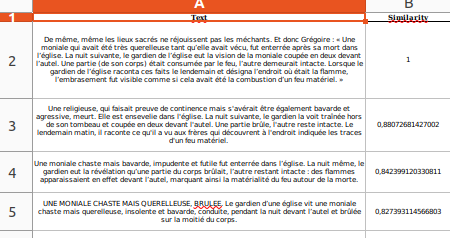
\includegraphics[width=0.7\linewidth]{images/similarite1.png}}
	\caption{Essai de comparaison}
\end{figure}

Malgré ces résultats encourageants, j'ai finalement décidé de renoncer à l'utilisation de l'IA pour trouver des correspondances entre les textes des deux bases de données. Cette décision s'explique par les nombreuses limitations rencontrées, notamment les problèmes de traduction, la lenteur des analyses, et la difficulté à définir ce qu'est un \textit{exemplum} : une forme littéraire complexe et fluide, difficile à cerner tant par un humain que par un algorithme\footcite{berliozIntroductionGenerale2010}. De plus, les \textit{exempla} présents dans les \index{Encyclopédies}encyclopédies diffèrent souvent de ceux répertoriés dans ThEMA, rendant la tâche encore plus ardue pour une IA. Un exemple illustrant cette difficulté est un \textit{exemplum} retrouvé dans la \textit{Summa de exemplis ac similitudinibus rerum} de Giovanni da San Gimignano, où l'auteur reprend une idée d'Aristote sur la nécessité de cultiver son cœur pour produire de bons fruits\footcite{RecitExemplaireUtilise}. Ce récit n'a trouvé aucun équivalent exact dans le corpus de ThEMA, le texte le plus proche présentant seulement 70\% de similarité. \\

\begin{figure}[H]
	\centering
	\fbox{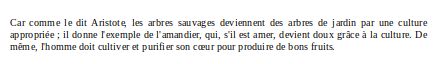
\includegraphics[width=0.8\linewidth]{images/textrecherche.png}}
	\caption{\textit{Exemplum} repéré dans SourcEncyMe}
\end{figure}

\begin{figure}[H]
	\centering
	\fbox{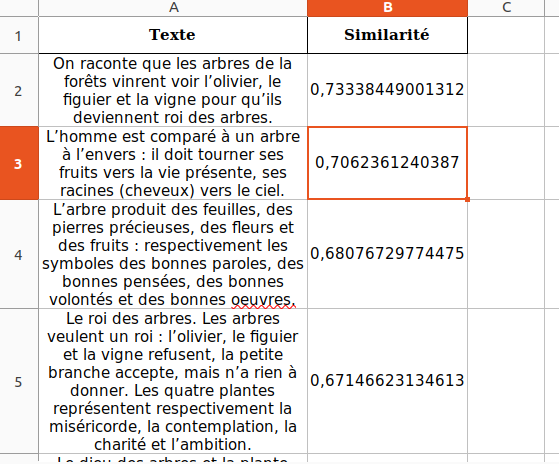
\includegraphics[width=0.6\linewidth]{images/similitude2.png}}
	\caption{Comparaison de l'\textit{exemplum} avec les récits exemplaire de ThEMA}
\end{figure}

Ainsi, j'ai préféré adopter une approche plus simple : repérer semi-manuellement les \textit{exempla} dans les encyclopédies. Contrairement à ThEMA, où les liens avec les encyclopédies ont été établis lors de l'indexation, ces \textit{exempla} n'ont pas encore été identifiés dans les \index{Encyclopédies}encyclopédies. L'entraînement d'un modèle de langage pour reconnaître un \textit{exemplum} aurait été une solution intéressante, mais il aurait fallu surmonter à nouveau les défis précédemment présentés.


\section{Identification des \textit{exempla} via des mots-clés}
Face à ces défis, il est apparu que l'utilisation d'une méthode plus ciblée pourrait s'avérer plus efficace. C'est ainsi que j'ai opté pour l'application de mots clés spécifiques. Cette méthode repose sur une caractéristique fréquente des \index{Récits exemplaires}récits exemplaires : ils sont souvent introduits par des termes latins comme « audivi », « legi », « memini », « verum », « dicitur », « narrat », « memini » ou « vidi »\footcite{bremondclaudeExemplum1982}. Cependant, tous ces mots n'ont pas été retenus, car dans les œuvres encyclopédiques, ils sont souvent utilisés dans d'autres contextes, notamment pour citer des œuvres ou des auteurs.

Par conséquent, je me suis concentré sur les mots les plus directement liés aux \textit{exempla} : « exemplum », « exempla », « exemplo », et « exemplis ». Cette approche par mots-clés m'a permis de contourner les difficultés liées à l'intelligence artificielle tout en offrant une méthode efficace pour identifier les \textit{exempla} dans les textes encyclopédiques.

De ce fait, avec une feuille de style \index{XSL}XSL, c'est-à-dire une page de code utilisée pour transformer et présenter des documents \index{XML}XML, j'ai créé un code qui, lorsqu'il rencontre l'une des déclinaisons d'\textit{exemplum} dans la balise <quote> du \index{XML}XML (c'est-à-dire là où se trouve le texte), balise le mot avec un marqueur et crée ensuite une balise <bibl>, si nécessaire, au-dessus de <quote> pour indiquer qu'il y a un \textit{exemplum}. Voilà ce que fait la transformation : \\

\begin{lstlisting}[breaklines=true]
	<cit n="7" xml:id="cit_idp82718352">
		<quote>Sexto, quia malus seruus cupidus existens, bona Domini in proprium usum vertit. Exemplum de seruo <name type="personne">Elisei</name>, et hoc pertinet ad simoniacos, qui bona Domini, id est,dona Spiritus sancti, pro sua utilitate temporali emunt, et vendunt.
		</quote>
	</cit>
\end{lstlisting}

\

\begin{lstlisting}[breaklines=true]
	<cit n="7" xml:id="cit_idp82718352">
		<bibl>
			<ref cert="low" target="#exemplum">Exemplum</ref>
		</bibl>
		<quote>Sexto, quia malus seruus cupidus existens, bona Domini in proprium usum vertit. <seg type="marqueur">Exemplum</seg> de seruo <name type="personne">Elisei</name>, et hoc pertinet ad simoniacos, qui bona Domini, id est, dona Spiritus sancti, pro sua utilitate temporali emunt, et vendunt.
		</quote>
	</cit>
\end{lstlisting}

\

Au départ, je souhaitais que ce code fonctionne uniquement lorsque les déclinaisons du mot « exemplum » se trouvent en début de phrase, car j'avais remarqué que c'est souvent dans ces cas-là que l'on a affaire à un véritable \textit{exemplum}. Cependant, après discussion avec \index{Isabelle Draelants}Isabelle Draelants et \index{Emmanuelle Kuhry}Emmanuelle Kuhry, cette approche a été abandonnée car elle risquait de laisser de côté certains récits exemplaires. Le choix a été fait d'effectuer un repérage plus large, quitte à avoir plus d'erreurs (annexe H), ce qui a nécessité un travail de vérification.

Prenons l'exemple de l'\index{Encyclopédies}encyclopédie de Giovanni da San Gimignano. Mara Calloni avait initialement identifié 220 \textit{exempla} en lisant le texte. Le code, pour sa part, en a détecté plus de 650. Après vérification par mes soins, le nombre exact d'\textit{exempla} est de 479. Bien que ce chiffre puisse sembler élevé, il est important de noter que l'ensemble de l'œuvre encyclopédique de San Gimignano est moralisée\footcite{oldoniGiovanniSanGimignano1994}. Le code repère donc un plus grand nombre d'\textit{exempla} que la lecture humaine, mais il se concentre uniquement sur les déclinaisons du mot \textit{exemplum}. En revanche, le repérage manuel effectué par Mara, qui ne faisait aucune discrimination dans les citations, a permis de déceler des \textit{exempla} même lorsqu'ils ne sont pas explicitement introduits par ces déclinaisons. Toutefois, l'ajout de mots introductifs supplémentaires pour affiner la recherche augmenterait considérablement la charge de travail pour la vérification, qui prenait déjà une quinzaine d'heures rien que pour les déclinaisons du mot \textit{exemplum}. Il est donc essentiel de déterminer jusqu'où nous sommes prêts à aller dans ce processus de vérification, car autrement, cela reviendrait presque à effectuer une recherche par lecture. Cela dit, cette méthode facilite le balisage, puisqu'il suffit ensuite de supprimer les éléments qui ne correspondent pas à un \textit{exemplum}.

C'est surtout avec le mot \textit{exemplum} que le plus grand nombre de \index{Récits exemplaires}récits exemplaires ont été trouvés (140), suivi par \textit{exemplo} (30), \textit{exempla} (13) et \textit{exemplis} (5). Cette répartition s'explique aisément. \textit{Exemplum} (nominatif singulier) est la forme de base du mot en latin\footcite{PageDedieeAu2024}. Elle est souvent utilisée pour introduire un récit exemplaire en tant que concept ou titre. \textit{Exemplo} (ablatif ou datif singulier) est fréquemment utilisé dans les constructions syntaxiques pour indiquer le moyen ou la cause (par exemple, « par un exemple », « grâce à l'exemple de... »)\footcite{PageDedieeAu2024}. Cette forme est souvent intégrée dans des phrases qui illustrent ou justifient un point par l'utilisation d'un exemple, ce qui la rend très présente dans les textes qui visent à enseigner ou moraliser.